%!Mode:: "TeX:UTF-8"
\documentclass[a4paper,12pts]{article}

\usepackage[polish]{babel}
\usepackage[utf8]{inputenc}
\usepackage{fontspec}
\setmainfont{Calibri}

\linespread{1.15}

\usepackage{caption}
\captionsetup{%
	font={footnotesize},
	labelfont={bf}
}

\usepackage{anysize}
\usepackage{geometry}

\usepackage{graphicx}

% Plik szablonowy do wykorzystania pózniej - nie zmieniaj go!

\begin{document}
	\thispagestyle{empty}
	\begin{flushleft}
		Wydział Elektrotechniki, Automatyki, Informatyki i Inżynierii Biomedycznej \\
		Informatyka, rok II \\
		Zespół numer 3 \\
		Piotr Kucharski \\
		Dominik Zabłotny \\
		\vspace*{\fill}
		%-----------NUMER CWICZENIA--------%
		{\large \textbf{Sprawozdanie z ćwiczenia nr 51} } \\
		%-----------TEMAT ĆWICZENIA--------%
		Współczynnik załamania światła dla ciał stałych.		
		\vfill	
		%-----------DATA-------------%
		15 listopada 2017 r
	\end{flushleft}
	
	\newpage
	
%--------------------------------------------------------------------------------------------------------------
	
	\section{Cel ćwiczenia}
	
	Celem wykonywanego ćwiczenia jest wyznaczenie współczynnika załamania światła dla szkła i zbadanie jego zmian w zależności od długości fali światła padającego.

%--------------------------------------------------------------------------------------------------------------	
	
	\section{Wstęp teoretyczny}
	
	Światło padające na granice dwóch ośrodków ulega dwóm zjawiskom, odbiciu i załamaniu.
	
	\subsection{Prawo odbicia}
	
	Jeżeli światło pada na granicę dwóch ośrodków, to ulega zarówno odbiciu na powierzchni granicznej, jak i załamaniu przy przejściu do drugiego ośrodka tak, jak pokazano to na Rys. 1 dla powierzchni płaskiej.
	
	\begin{figure}[!h]
		\centering
		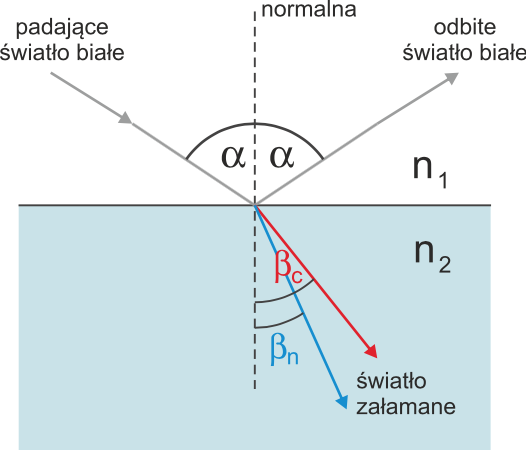
\includegraphics[scale=0.3]{odbicie.png}
 		\caption{Schemat Prawa Odbicia \\ źródło: OPEN e-Podręczniki AGH - ,,Prawo odbicia i załamania"}
		\label{odbicie}
	\end{figure}
	
	\subsection{Prawo załamania}
	
	Prawo załamania (tzw. Prawo Snellius'a) definiuje stosunek sinusa kąta padania do sinusa kąta załamania, który jest równy stosunkowi bezwzględnego współczynnika załamania ośrodka pierwszego $n_1$, czyli współczynnikowi zględnego załamania światła ośrodka drugiego względem pierwszego. Kąty padania i załamania leżą w tej samej płaszczyźnie. Współczynnik załamania zależy od długości fali światła padającego. Po kilku przekształceniach trygonometrycznych otrzymujemy wzór:
	
	\begin{equation}
		\frac{sin\alpha}{sin\beta} = \frac{V_1}{V_2} = \frac{\lambda_1}{\lambda_2} = n = const
	\end{equation} 

	gdzie $\alpha$ to kąt padania, $\beta$ kąt załamanej wiązki światła, n to współczynnik załamania światła ośrodka drugiego względem pierwszego.

%--------------------------------------------------------------------------------------------------------------
	
	\section{Układ pomiarowy}
	
	Układ pomiarowy składa się z:
	
	\begin{itemize}
		\item Mikroskop wyposażony w czujnik mikrometryczny i nasadkę krzyżową,
		\item Śruba mikrometryczna,
		\item Zestaw płytek wykonanych z pleksiglasu oraz ze szkła, różnej długości.
	\end{itemize}
	
%--------------------------------------------------------------------------------------------------------------
	
	\section{Wykonanie ćwiczenia}
	
	Schemat wykonania ćwiczenia:
	
	\begin{itemize}
		\item Wykonanie pomiaru grubości płytek wykonanych z pleksiglasu i szkła za pomocą śruby mikrometrycznej,
		\item Zamocowanie badanej płytki w uchwycie na stoliku mikroskopu,
		\item Odczyt wartości przesunięcia czujnika mikrometrycznego $a_g$,
		\item Wykonanie odczytów dla kolejnych płytek.
	\end{itemize}
	
%--------------------------------------------------------------------------------------------------------------
	
	\section{Opracowanie danych pomiarowych}
	
	%----------------------------------------------------------------------------------------------------------	
	
	\subsection{Analiza niepewności}
	
%--------------------------------------------------------------------------------------------------------------

	\section{Podsumowanie}

%--------------------------------------------------------------------------------------------------------------

\end{document}